
%%*************************************************************************
%%
%% Analysis of Biosignals by Biologically Inspired Algorithms
%% V1.0
%% 2011/05/05
%% by Peter Boraros
%% See:
%% http://www.pborky.sk/contact
%% for current contact information.
%%
%% Desription goes here.
%%
%%
%%*************************************************************************
%% Legal Notice:
%%
%% This code is offered as-is without any warranty either expressed or
%% implied; without even the implied warranty of MERCHANTABILITY or
%% FITNESS FOR A PARTICULAR PURPOSE! 
%% User assumes all risk.
%%
%% This work by Peter Boraros is licensed under a 
%% Creative Commons Attribution-NonCommercial-ShareAlike 3.0 Unported License.
%% http://creativecommons.org/licenses/by-nc-sa/3.0/

\documentclass[a4paper]{IEEEtran}

\usepackage{cite}
% \usepackage[nocompress]{cite}
\usepackage{ifpdf}

\ifpdf
\usepackage[pdftex]{graphicx}
\graphicspath{{./img/}}
\DeclareGraphicsExtensions{.pdf}
\else
\usepackage[dvips]{graphicx}
\graphicspath{{./img/}}
\DeclareGraphicsExtensions{.eps}
\fi

\usepackage[cmex10]{amsmath}
\usepackage{amsfonts}
\usepackage{amssymb}
\interdisplaylinepenalty=2500

\usepackage{algorithmic}

\usepackage{array}

\usepackage{mdwmath}
\usepackage{mdwtab}

\usepackage{eqparbox}

\usepackage[hang,small,center,bf]{caption}
% \usepackage[tight,normalsize,sf,SF]{subfigure}
%\usepackage[tight,footnotesize]{subfigure}
\usepackage{subfig}
% \usepackage[caption=false,font=normalsize,labelfont=sf,textfont=sf]{subfig}
% \usepackage[caption=false,font=footnotesize]{subfig}

\usepackage[utf8x]{inputenc}
\usepackage{url}
\usepackage{fixltx2e}
\usepackage{stfloats}
\usepackage{ucs}
\usepackage{multirow}

% correct bad hyphenation here
\hyphenation{op-tical net-works semi-conduc-tor}

\renewcommand{\labelitemi}{$\bullet$}
\renewcommand{\labelitemii}{$\circ$}
\renewcommand{\labelitemiii}{$\ast$}

\setlength{\textheight}{260mm}

\begin{document}
\title{Analysis of biosignals by means of\\ biologically inspired algorithms}
\date{May 29, 2011}
\author{Peter~Boraros %
\thanks{{Peter Boraros}, Czech technical university, Faculty of Electrical Engineering,
see~\texttt{http://www.pborky.sk/contact} for a contact infomation}}%

% The paper headers
\markboth{Peter Boraros, Czech technical university, Faculty of Electrical Engineering, Prague, Czech Republic}{}

\IEEEcompsoctitleabstractindextext{%
\begin{abstract}
The aim of this document is to show the usage of biologically inspired algorithms
in analysis of facial electromyography and electroencephalography.
Concretelly, it depicts the process of obtaining data, preprocessing using fast fourier
transform and classifing by means of a self-organizing map. 
Searching through the parameter space in order to find proper parametrisation of whole
classification process is performed by a genetic algorithm. All source code has been
published at \cite{biosiglab}.
\end{abstract}}

\maketitle
\IEEEdisplaynotcompsoctitleabstractindextext
\IEEEpeerreviewmaketitle


\section{Introduction}
\IEEEPARstart{T}{}he goal is to implement methods for analysis of
a electromyography (EMG) and a electroencephalography (EEG)
in order to allow an estimation of the subject`s mimics, 
feelings or enable ability to classify the sleep stages and eventually control 
external equipment during a specific sleep stage.

This work depicts an usage of a self-organizing maps (SOM) as well as the usage of a genetic
algorithms (GA). It is possible to use other recognition or optimalization
techniques but usage of mentioned 
methods was induced by project assignment at a school course ``Biologically inspired 
algorithms''.

The self-ogranizing map is used  at this experiment as the method of feature recongnition in 
supervised mode. The genetic algorithm is used to estimate the proper parametrization of 
whole classification process. It searches through possible parameter ranges and 
depending on a value of fitness it chooses the best configuration. The fitness function
models a objectives of optimalization.

The next research ought to be oriented on a genetic programming. The genetic programming 
is the method of construction a computer program by similar way like the genetic
algorithm. Both are inspired by the nature and the process of evolution.

%Software used by this available at \url{https://github.com/pborky/biosiglab}.

\subsection{A training data, preprocessing}
The training data is usually a pulse-code modulated (PCM) signal \cite{pcm} along with a
classification information attached during the signal gathering.
A sampling frequency, can be reduced by averaging particular number of samples. Classification
information is then reduced by electing a most frequent classes in a given set.
Reduction is optional, it lowers the resolution but also lowers the
computational complexity. Compromise ought to be found.

The signal has to be transformed
from a time domain to a frequency domain. %TODO: really??
This can be achieved by fourier-related tranforms, e.g. by a fourier\cite{fourier} or
a wavelet\cite{wavelet} transform.
The wavelet transform, unlike the fourier transform, captures not only a notion of the 
frequency content of the input, by examining it at different scales, but also temporal content.
Only the fast fourier transform has been used in this work.

Before the fourier transform, the PCM signal is choped into overlaping slices (windows).
The transform ought to be aplied to each slice resulting in a complex spectral components.
Phase information is usually discarded.
%TODO:describe possible other methods

Next the resulting vectors are subject to reduction by means of a
frequency filtering. Frequency filters are problem dependent.
The \textit{figure~\ref{fig:filters2}} shows aproximate ranges for some widely used bioelectric signals.
\begin{figure}[h]
	\centering
	\includegraphics[width=80mm]{filters2}
	\caption{Frequency ranges of some types of bioelectric signals}
	\label{fig:filters2}
\end{figure}

Fitered spectral components are subject to normalisation/equalisation
in order to put the components
in the scale. There are several algorithms to choose. Analysed choices are:
histogram~\cite{hist}, logistic or logaritmic normalisation
with scaling the values between $ \langle 0, 1 \rangle $ or a variance normalisation,
that scales variables linearly such that their variance is equal~to~1.

\subsection{Self-organizing map}
The normalised training data is passed to train the self-organising map.
The self-organising map is a type of artificial neural network that is
trained using unsupervised learning to produce a low-dimensional 
(typically two-dimensional), discretized representation of the input 
space of the training samples, called a map. It is method of vector 
quantisation that can be used to cluster analysis.
The self-organizing map consists of components called nodes or neurons. 
Associated with each node is a weight vector of the same dimension 
as the input data vectors and a position in the map space.
The usual arrangement of nodes is a regular spacing in a hexagonal or rectangular grid. 
%More detailed information about used algorithms is available at \cite{somtoolbox}. 
The neurons with weight vectors most similar to the inputs are called 
the best matching units (BMUs).

There are two ways to interpret a SOM. 
Because in the training phase weights of the whole neighborhood are moved in the 
same direction, similar items tend to excite adjacent neurons. Therefore, 
SOM forms a semantic map where similar samples are mapped close together 
and dissimilar apart. This may be visualized by a U-Matrix 
(Euclidean distance between weight vectors of neighboring cells) of the SOM.

The other way is to think of neuronal weights as pointers to the input space. 
They form a discrete approximation of the distribution of training samples.
More neurons point to regions with high training sample concentration and 
fewer where the samples are scarce~\cite{somwiki}.

This unsupervised process can be commuted to a supervised by adding a classification
information before process.
The class information is then encoded using 1-of-N encoding and appended to the 
spectral vectors. After training, the class of each map unit
is determined by taking maximum over these added components.
Finally the class information is removed~\cite{somtoolbox}.

The quality of output is controled by several parameters. The most important are 
training algorithm, maps size and topografic layout and lattice.

The spatial layout of topological surface has to be checked by means of a projection
of the weight vectors to the euclidean space using dimensionality reduction algorithms
such as principal component analysis.
It should not contain irregularites, the surface ought to be ``flat''.
To quantify this criterion a tolopological error is defined. It is the proportion 
of all data vectors for which first and second BMUs are not adjacent units.

Another criterion is a validation/testing error. Traning set is divided into $ k $-folds
and it is trained using $ k-1 $ folds. Error is determined using the remaining fold.
This is repeated for each fold. An average error is then the subject to minimalisation.

\subsection{Genetic algorithm}
A genetic algorithm (GA) is a search heuristic that mimics the 
process of natural evolution. This heuristic is routinely used to 
generate useful solutions to optimization and search problems.

In a genetic algorithm, a population of strings (called chromosomes), 
which encode candidate solutions (called individuals) to an optimization problem,
evolves toward better solutions.
Traditionally, solutions are represented in binary as strings of 0s and 1s, 
but other encodings are also possible. 
The evolution usually starts from a population of randomly generated individuals 
and happens in generations.
In each generation, the fitness of every individual in the population is evaluated,
multiple individuals are stochastically selected from the current population 
(based on their fitness), and modified (recombined and possibly randomly mutated) 
to form a new population. The new population is then used in the next 
iteration of the algorithm. 
Commonly, the algorithm terminates when either a maximum number of generations 
has been produced, or a satisfactory fitness level has been reached 
for the population. 
If the algorithm has terminated due to a maximum number of generations, 
a satisfactory solution may or may not have been reached.

A typical genetic algorithm requires:
\begin{itemize}
	\item a genetic representation of the solution domain,
	\item a fitness function to evaluate the solution domain.
\end{itemize}
A standard \textit{representation} of the solution is as an array of bits. 
Arrays of other types and structures can be used in essentially the same way. 
The main property that makes these genetic representations convenient 
is that their parts are easily aligned due to their fixed size,
which facilitates simple crossover operations. It is possible to 
represent solution by other techniques like variable array representation,
trees or graphs but the operations are more complex in that case.
The \textit{fitness function} is defined over the genetic representation and
measures the quality of the represented solution. The fitness function 
is always problem dependent.

Genetic programming (GP) is an evolutionary algorithm based methodology 
inspired by biological evolution to find computer programs that perform 
a user-defined task. 
It is a specialization of genetic algorithms (GA) where each 
individual is a computer program. 
It is a machine learning technique used to optimize a population of 
computer programs according to a fitness landscape determined by a 
program's ability to perform a given computational task \cite{gawiki}.


\section{Experiments}
\label{sec:ex}
\subsection{Training data} 
\label{sec:ex_train_data}
An equipment used for this experiments is {Nia game controller}, made by 
{OCZ Techologies}. This device provides a HID standard interface.
After it is connected, it starts to send 24-bit PCM samples, 
sampled at frequency 4kHz. The device has only one balanced channel, thus 
it is not possible to preform complex analysis of neural signals,
however for detection of the EMG or the EOG signal it is sufficient.

The training information is attached during a process of data gathering by a human operator 
through a GUI application.
The PCM data from device is saved along with the class information from the
user interface.

The training data contains features of facial mimics. In this experiments
following classes of grimaces have beem recorded: eye-wink (left, right, both), 
relax (no grimace).
Recording time is about up to 3 minutes

\subsection{Self-organizing map}
\label{sec:ex_som}
This experiment uses implemetation of the SOM based on \cite{somtoolbox}.
This implementation has wide set of options and algorithms.

Following options were analysed:
\begin{figure}[!b]
	\centering
	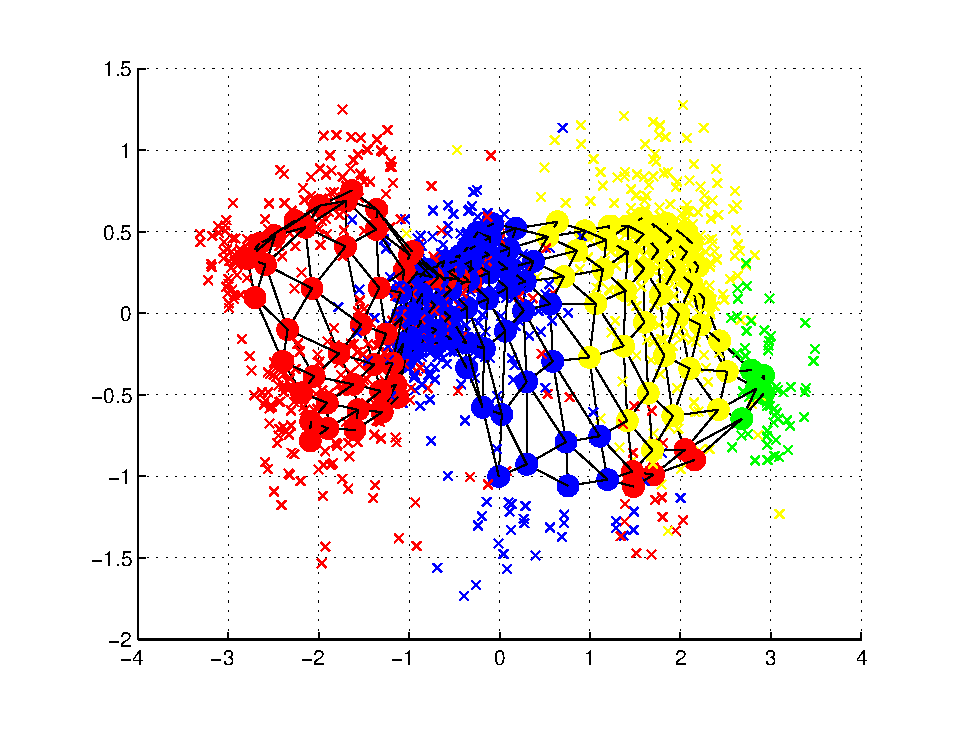
\includegraphics[width=80mm]{som_topol_proj}
	\caption{The PCA projection of the topology of the self-organizing map along with the data}
	\label{fig:som_topol_proj}
\end{figure}
\begin{itemize}
	\item usage of \textit{batch} or \textit{sequential} training algorithm 
	\cite{somtoolbox},
	\item \textit{hexagonal} or \textit{rectangular} lattice of the map,
	\item size of the map - the default number of map units is determined by heuristic formula 
	$ n_{units} = 5\cdot {n_{data}}^{0.54321} $. \textit{Small} map then
	has $ 0.25\cdot n_{units} $ and \textit{big} map has $ 4\cdot n_{units} $. Only
	\textit{small} and \textit{normal} size have been analysed.
\end{itemize}

The \textit{figure~\ref{fig:som_topol_proj}} depicts the trained self-organizing map and the traning data.
It is a  projection of input data vectors and best matching units using an principal component analysis~\cite{pca}.
This projection reduces a dimensionality of the vectors by linear tranformation using a principal eigenvectors.
Different projection, a Sammon projection~\cite{sammon}, is depicted on the \textit{figure \ref{fig:som_samon_proj}}.
It is an nonlienar projection, that finds an low dimensional model iteratively,
trying to keep euclidean distances between objects from the high dimesional space.
Convergent solutions are not allways guaranteed.

\begin{figure}[!h]
	\centering
	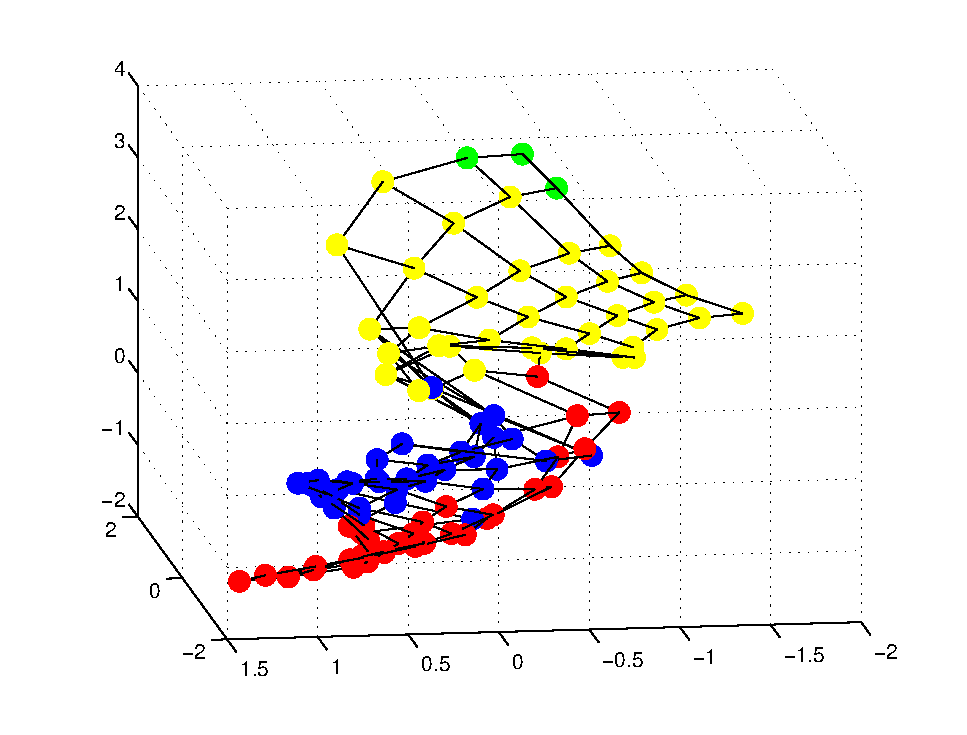
\includegraphics[width=80mm]{som_samon_proj}
	\caption{The Sammon projection of the topology of the self-organizing map}
	\label{fig:som_samon_proj}
\end{figure}

The \textit{figure~\ref{fig:som_umat}} shows two-dimensional projection of the best matching units and
a labeling information.
Color of elements of the U-matrix represents the distance between best matching units. Lighter color
means larger distance and usually it depicts the division between clusters.
The division between the red and blue cluster is not clearly observable on the \textit{fig. \ref{fig:som_umat}},
but see \textit{fig. \ref{fig:som_umat_2}} for a better example.
The labeling information is classification of best matching units. Color of labeling is following (same coloring is used
for the PCA and Sammon projection as well):
\begin{itemize}
	\item red - relax,
	\item green - wink (both eyes),
	\item blue - right eye wink,
	\item yellow - left eye wink.
\end{itemize}

Figured solution has been evaluated as a best-fit solution by the genetic algorithm.
\begin{figure}[!h]
	\centering
	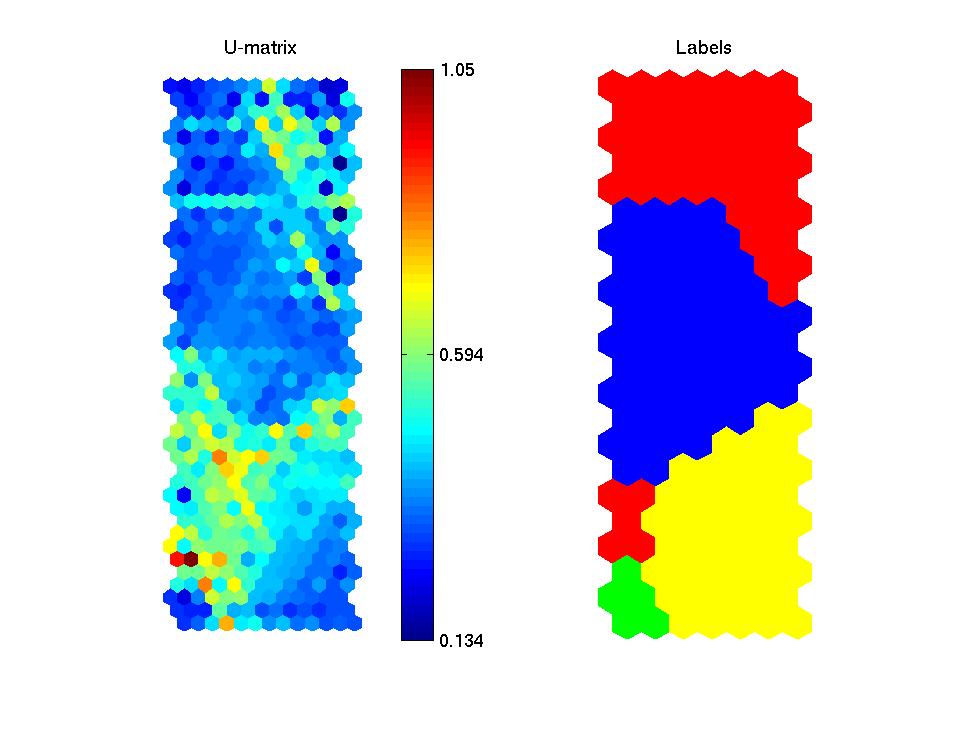
\includegraphics[width=80mm]{som_umat}
	\caption{The U-matrix and classification of best matching units}
	\label{fig:som_umat}
\end{figure}

\subsection{Search space}
\label{sec:ex_search}
The whole process is controlled by several parameters.
The parameters can be determined by way of searching the search space.
Following parameters have been identified:
\begin{itemize}
	\item sampling frequency ($ f_{samp} $),
	\item time window before the fourier transform ($ n_w $),
	\item overlap of the time windows ($ n_o $),
	\item frequency filtering after the fourier tranform process (interval $ \langle f_l, f_h
	\rangle $ defines portion of signal that is kept),
	\item normalisation method (\textit{histogram}, \textit{logaritmic}, 
	\textit{range}, \textit{logistic}),
	\item SOM training algorithm (\textit{batch} or \textit{sequential}),
	\item lattice of the SOM (\textit{hexagonal} or \textit{rectangular}),
	\item size of the SOM (depends on size of traning dataset).
\end{itemize} %
The values of the parameters are listed  in the \textit{table \ref{tbl:searchspace}}.
\begin{table}[!h]
\caption{The search space}
	\begin{center}
		\begin{tabular}{|l|| l |}
			\hline
			degree of freedom & values \\
			\hline
			\hline
			$ f_{samp} [Hz] $ & 256, 666, 1333, 4000\\
			\hline
			$ n_w $ & 80, 200, 800, 2000 \\
			\hline
			$ n_o $ & 2, 8 \\
			\hline
			$ \langle f_l[Hz], f_h[Hz] \rangle $ & $ \langle 0, 50\rangle $,  
			$ \langle 20, 250\rangle $  \\
			\hline
			normalisation & histogram, logaritmic, variance, logistic \\
			\hline
			training algorithm & batch, sequential  \\
			\hline
			map lattice & hexagonal, rectangular \\
			\hline
			map size  & small, normal \\
			\hline
		\end{tabular}
	\end{center}
\label{tbl:searchspace}
\end{table}

The objectives of optimalisation token in account are:
\begin{itemize}
	\item validation error $ e_v $ of the trained SOM network evaluated by k-fold
	crossvalidation, $ e_v \in \langle 0, 1 \rangle $,
	\item topological error  $ e_t $ of the trained SOM using whole dataset,
	$ e_t \in \langle 0, 1 \rangle $,
	\item window size $ \Delta t_w $ ,
	\item run time $ t_r $.
\end{itemize}
\begin{figure*}[!h] %
  \centering
  \subfloat[Time window width]{\label{fig:fit_ev}\includegraphics[width=44mm]{fit_ev}}
  \subfloat[Topological error]{\label{fig:fit_et}\includegraphics[width=44mm]{fit_et}}
  \subfloat[Time window width]{\label{fig:fit_tw}\includegraphics[width=44mm]{fit_tw}}
  \subfloat[Run time]{\label{fig:fit_tr}\includegraphics[width=44mm]{fit_tr}}
  \caption{The fitness function partial graphs}
  \label{fig:fit}
\end{figure*}
The fitness function has been choosen empirically based on optimalization objectives:
\[ f = -\ln(e_v+10^{-2 }) - \ln(\Delta t_w+0.5) - (0.7\cdot e_t-0.7) - P(t_r) \]
where:\\
$ P(t) $ is sigmoid function defined as:
\[ P(t) = \frac{5}{1+10\cdot e^{6-0.15t}} \]
$ e_v $ is validation error,\\
$ e_t $ is topological error,\\
$ t_r $ is run time,\\
$ \Delta t_w $ is window time span and it can be expressed as 
\[  \Delta t_w = \frac{n_w}{f_{samp}}  \]
where:\\
$ n_w $ is number of samples within window,\\
$ f_{samp} $ is sampling frequency.
\\

Impact of particular objectives on value of the fitness is following:
\begin{itemize}
	\item validation error (\textit{fig.~\ref{fig:fit_ev}}) is the key objective and thus its impact
	on the fitness function is maximal ($ -\ln(e_v+10^{-2 }) $),
	\item topological error (\textit{fig.~\ref{fig:fit_et}}) describes a quality 
	of the SOM ($ -(0.7\cdot e_t-0.7) $),
	\item time window (\textit{fig.~\ref{fig:fit_tw}}) has an impact on a time resolution
	of the classification ($ -\ln(\Delta t_w+0.5) $),
	\item run time  (\textit{fig.~\ref{fig:fit_tr}}) should not exceed one minute thus 
	the sigmoid function $ - 5 \cdot (1+10\cdot e^{6-0.15t_r})^{-1} $ 
	models this case.
\end{itemize}

\subsection{Genetic algorithm}
\label{sec:ex_ga}
Choosen search space is discrete and it is listed  in \textit{table~\ref{tbl:searchspace}}.
The implementation of the genetic algorithm to be introduced at this place
has following properties:

\begin{itemize}
	\item genes:
	\begin{itemize}
		\item binary strings of different length,
		\item integer indices to the search space,
	\end{itemize}
	\item given initial population size,
	\item random uniform initialization,
	\item selection strategy:
	\begin{itemize}
		\item surviving species are selected using a stochastic universal 
		sampling reducing the population size up to given initial value,
	\end{itemize}
	\item crossover:
	\begin{itemize}
		\item parents for crossover are selected using a fitness proportionate
		selection of the surviving species,
		\item count of selection rounds is determined by empiric formula
		\[ N_{pr} = \lceil 0.35\cdot N_{survived} \rceil \] 		
		where $ N_{survived} $ is the number of survived species after stochastic selection.
		The value of $ N_{pr} $ limits the count of selected species.
		\item for each parent, its pair is selected by random,
		\item genes selected by random are swapped; it is uniform selection using 
		genes that are different; solution is accepted if
		produces  offsprings distinct from parents (i.e. at least one differing gene must be kept or swapped respectivelly),
	\end{itemize}
\end{itemize}
\begin{itemize}
	\item mutations:
	\begin{itemize}
		\item species for mutation are selected by 2 ways:
		\begin{itemize}
			\item from offsprings generated by crossover with probability of mutation for each one:
			$ P_{mo} = n_{mr} $.
			\item using an inversed-fitness proportionate
			selection from the surving species, where the inverse fitness is expressed as
			$ f'=-f  $
			and count of selection the rounds is
			\[ N_{mr} = \lceil n_{mr}\cdot N_{survived} \rceil \]
			where 
			$ n_{mr} $  is the rate of mutation in given population denoted as:			
			\[ n_{mr} = 0.05+\dfrac{0.25}{10\cdot e^{0.11\cdot i_{gen}-7}}\]
			where
			$ i_{gen} $ is the actual generation.
			The value of $ N_{mr} $ limits the count of selected species. 
			See \textit{fig.~\ref{fig:mut_r}} for graph of dependency of the rate of mutation  
			on the generation.
		\end{itemize}
		\item each bit is flipped with fixed probability
		$ P_{mb} = 0.2 $.
	\end{itemize}
\end{itemize}
\begin{itemize}
	\item stop condition:
	\begin{itemize}
		\item fitness of a best-fit specie for given interval of generations has not been changed.
	\end{itemize}	
\end{itemize}
\begin{figure}[!h]
	\centering
	\includegraphics[width=80mm]{mut_r}
	\caption{Dependency of the mutation rate on the generation.}
	\label{fig:mut_r}
\end{figure}

\subsection{Measurements}
Values listed in the \textit{table~\ref{tbl:somagrresults}} are representing distribution of the fitness
over changing parameters.
Statistical charecteristics, such as minimal, maximal or mean value or standard deviation, have been calculated
over all possible configurations with one particular parameter fixed.
The \textit{table~\ref{tbl:somresults}} lists measurements of fitness for five best-fit 
and one of the worst-fit configurations.
Internal states of the classifier (i.e. weight vectors of self-organizing map)
have been plotted on \textit{figures \ref{fig:som_topol_proj}, \ref{fig:som_samon_proj}, \ref{fig:som_umat}, 
\ref{fig:som_config_2}, \ref{fig:som_config_5}} and \textit{\ref{fig:som_config_6}}, for configurations listen in 
the \textit{table \ref{tbl:somresults}}.


\begin{figure*}[!t]
	\centering
	\subfloat[Single run of the genetic algorithm]
		{\label{fig:conv_curve_s}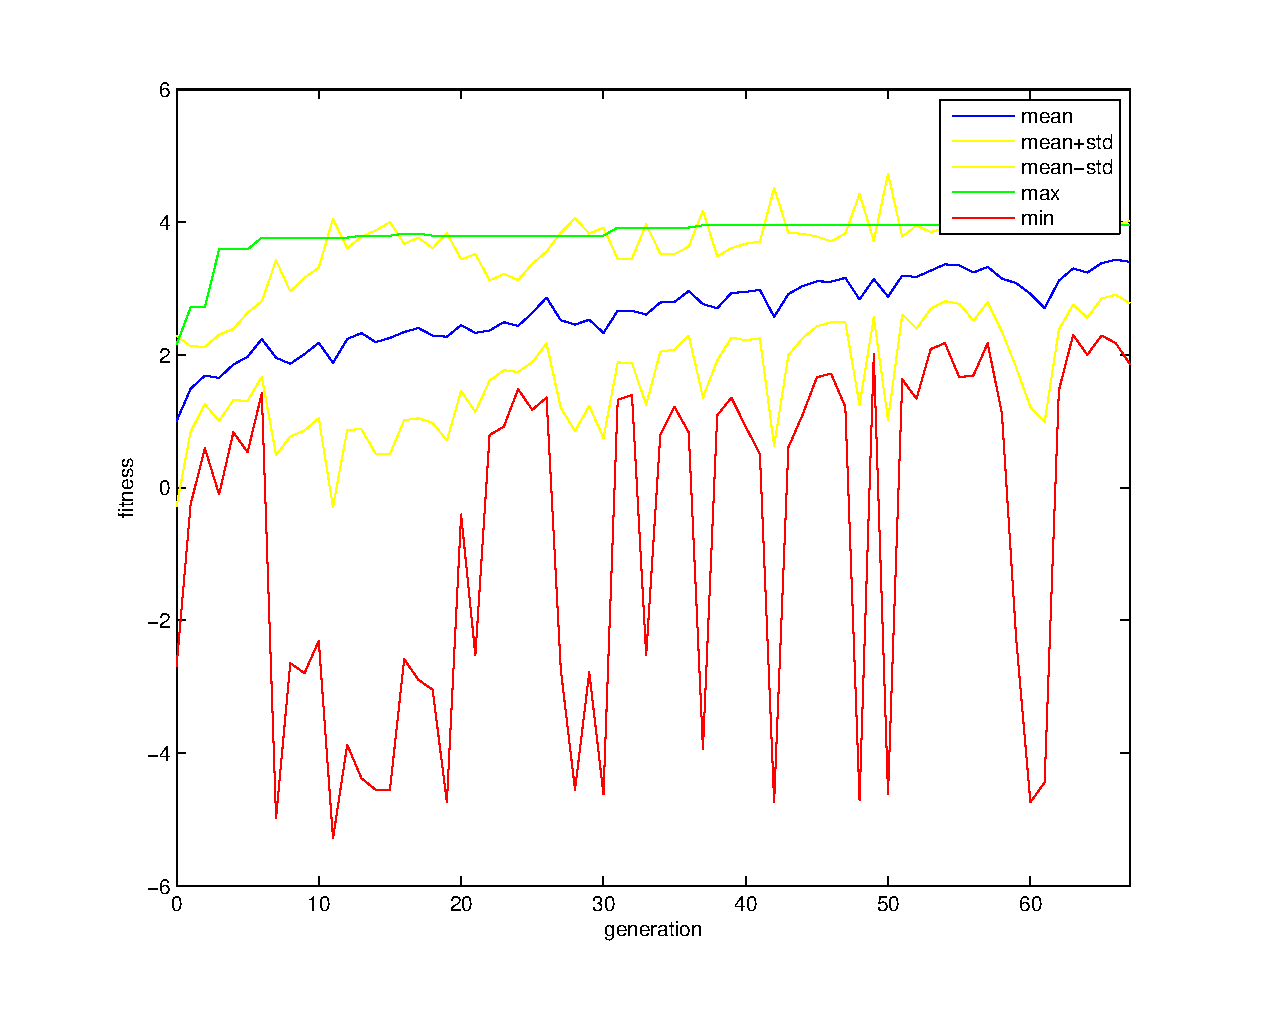
\includegraphics[width=90mm]{ga_conv_curve_s}}	
	\subfloat[Agregated over 100 runs with limit of 150 generations.]
		{\label{fig:conv_curve}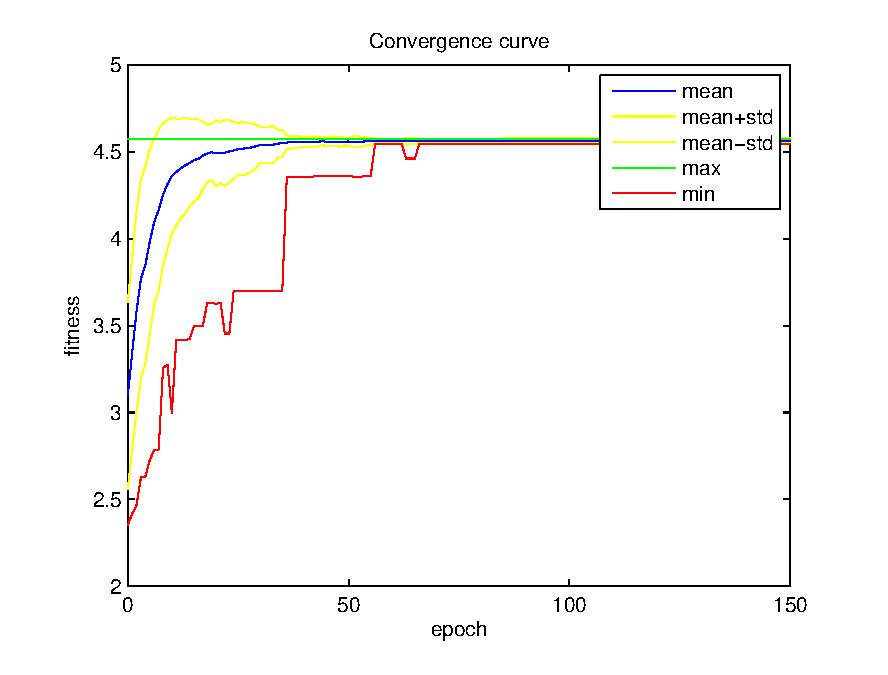
\includegraphics[width=90mm]{ga_conv_curve}}
	\caption{The convergence curves along with the population size}
	\label{fig:conv_curvx}
\end{figure*}
\begin{table*}[!h]
\caption{Measures of choosen configurations}
	\begin{tabular}{|c||p{8mm}|p{8mm}|p{4mm}|p{4mm}|m{5mm} |p{8.5mm}|p{7mm}|p{8mm}|p{11mm} ||p{10mm}|p{10mm}|p{10mm}|p{10mm}|p{10mm}|}
		\hline
			\multirow{2}{*}{\textbf{No}} & 
			\multicolumn{9}{c||}{\textbf{Parameters}} & 
			\multicolumn{5}{c|}{\textbf{Measures}} \\
		\cline{2-15}
			&
			$ \mathbf{f_{samp}} $& 
			$ \mathbf{n_{wnd}} $& 
			$ \mathbf{n_o} $&
			$ \mathbf{f_l} $&
			$ \mathbf{f_h} $& 
			\textbf{norm}&
			\textbf{train}&
			\textbf{lattice} &
			\textbf{map~size} &
			\textbf{val.err.}&
			\textbf{top.err.}&
			\textbf{runtime}&
			\textbf{window}& 
			\textbf{fitness}\\
		\hline\hline
1 & 666 & 800 & 8 & 20 & 200 & logistic & batch & rect & normal & 0.00646 &  0.02586 &  5.21314 &  1.2 & 4.2550 \\ \hline
2 & 1333 & 800 & 2 & 20 & 200 & logistic & batch & hexa & normal &  0.01693 &  0.02966 &  1.50804 &  0.6 & 4.1968 \\ \hline
3 & 1333 & 800 & 2 & 20 & 200 & logistic & batch & rect & normal &  0.01694 &  0.02966 &  1.30751 &  0.6 & 4.1964 \\ \hline
4 & 1333 & 800 & 8 & 20 & 200 & hist & batch & hexa & normal &  0.01816 &  0.01495 &  4.24669 &  0.6 & 4.1616 \\ \hline
5 & 4000 & 2000 & 2 & 20 & 200 & logistic & batch & rect & normal &  0.02113 & 0.01760 &  1.17217 &  0.5 & 4.1556 \\ \hline
6 & 1333 & 800 & 8 & 20 & 200 & hist & seq & rect & normal & 0.03365 & 0.03953 & 18.8976 & 0.6 & 3.6875 \\ \hline
7 & 256 & 800 & 2 & 20 & 200 & logistic & batch & hexa & small &   0.30486 &    0 &   19.4080 &    3 &  0.5801 \\ \hline
8 & 256 & 800 & 8 & 20 & 200 & logistic & seq & hexa & normal & 0.09384 & 0 & 50.8771 & 3 & 0.0207 \\ \hline
	\end{tabular}
	\label{tbl:somresults}
\end{table*}


Statistical agregations over 100 runs of genetic algorithm are stated in the \textit{table~\ref{tbl:garesults}}.
A configuration has been considered to be winner if its measure of fitness has been best of last surviving population
after the genetic algorithm reached the stop condition. Run time is time elapsed by single run of genetic
algorithm until solution has been found.
A generation count is a number of generations that has been emerged till the stop condition has been reached.
\begin{table}[!t]
	\caption{Dependency of the fitness on values of parameters}
	\centering
	\begin{tabular}{|c|c||c|c|c|c|}
		\hline
			\multirow{2}{*}{\textbf{Parameter}} & 
			\multirow{2}{*}{\textbf{Value}} & 
			\multicolumn{4}{c|}{\textbf{Fitness}} \\ 
		\cline{3-6}
			& &
			\textbf{min} &
			\textbf{mean} &
			\textbf{std} &
			\textbf{max} \\
		\hline
		\hline
			\multirow{4}{*}{\parbox[c]{20mm}{\centering\textbf{samp. frequency}\\ $ \mathbf{f_{sampl}[Hz]} $}}
			& 256 & -5.3882 & 0.7539 & 2.1562 & 3.7107\\ \cline{2-6}
			& 666 & 0.1852 & 1.8198 & 0.6429 & 4.2550\\ \cline{2-6}
			& 1333 & 0.4574 & 1.9894 & 0.5854 & 4.1968\\ \cline{2-6}
			& 4000 & -3.7500 & 1.7250 & 1.0428 & 4.1556\\
		\hline
			\multirow{4}{*}{\parbox[c]{20mm}{\centering\textbf{window width}\\ $ \mathbf{n_w} $}}
			& 80 & -3.7500 & 1.6794 & 0.9686 & 2.9619\\ \cline{2-6}
			& 200 & 0.4445 & 1.8854 & 0.4932 & 3.7107\\ \cline{2-6}
			& 800 & -2.8073 & 1.8551 & 0.8120 & 4.2550\\ \cline{2-6}
			& 2000 & -5.3882 & 0.8682 & 2.2125 & 4.1556\\ 
		\hline
			\multirow{2}{*}{\parbox[c]{20mm}{\centering\textbf{window overlap}\\ $ \mathbf{n_o} $}}
			& 2 & -5.3882 & 1.5664 & 1.2777 & 4.1968\\ \cline{2-6}
			& 8 & -5.3445 & 1.5777 & 1.4405 & 4.2550\\
		\hline		
			\multirow{2}{*}{\parbox[c]{20mm}{\centering\textbf{frequency filter}\\$\mathbf{\langle f_l,f_h \rangle[Hz]}$}}
			& $ \langle 0, 50 \rangle $ & -3.7500 & 1.4637 & 0.6655 & 3.2315\\ \cline{2-6}
			& $ \langle 20, 200 \rangle $ & -5.3882 & 1.6804 & 1.8004 & 4.2550\\
		\hline
			\multirow{4}{*}{\parbox[c]{20mm}{\centering\textbf{normalization}\\ \textbf{method}}}
			& hist & -5.0890 & 1.6729 & 1.3765 & 4.1616\\ \cline{2-6}
			& log & -5.3882 & 1.2908 & 1.3005 & 2.6185\\ \cline{2-6}
			& variance & -5.1476 & 1.5529 & 1.3119 & 3.4393\\ \cline{2-6}
			& logist & -5.0324 & 1.7716 & 1.4091 & 4.2550\\
		\hline
			\multirow{2}{*}{\parbox[c]{20mm}{\centering\textbf{training}\\ \textbf{algorithm}}}
			& sequence & -5.3882 & 1.4589 & 1.4011 & 3.6875\\ \cline{2-6}
			& batch & -5.2988 & 1.6852 & 1.3111 & 4.2550\\
		\hline
			\multirow{2}{*}{\textbf{map lattice}}
			& hexa & -5.3445 & 1.5727 & 1.3672 & 4.1968\\ \cline{2-6}
			& rect & -5.3882 & 1.5714 & 1.3559 & 4.2550\\
		\hline
			\multirow{2}{*}{\textbf{map size}}
			& small & -5.3882 & 1.4177 & 1.2621 & 3.2344\\ \cline{2-6}
			& normal & -5.0296 & 1.7264 & 1.4378 & 4.2550\\
		\hline
	\end{tabular}
	\label{tbl:somagrresults}
\end{table}
\begin{table}[!t]
	\caption{Measures over 100 runs of the genetic algorithm}
	\centering
	\begin{tabular}{|c||r|r|r|r|}
		\hline
			\textbf{} &  \textbf{min} & \textbf{mean} & \textbf{std} &  \textbf{max} \\
		\hline
		\hline
		\textbf{winner`s fitness} & 4.1616 & 4.2450 & 0.0235 & 4.2550 \\ \hline
		\textbf{run time [sec]} & 778 & 4252 & 1166 & 7524 \\ \hline
		\textbf{population count} & 1.0000 & 23.8090 & 4.9113 & 34.0000 \\ \hline
		\textbf{generation count} & 32.0000 & 46.4800 & 11.5238 & 85.0000 \\ \hline
		\textbf{visited states} & 96 & 317 & 55 & 447 \\ \hline
	\end{tabular}
	\label{tbl:garesults}
\end{table}
A population count is a number of configurations in each particular generation. It has been computed over 
all 100 runs and all generations.
The states are considered to be visited once their fitness has been calculated.
A values stated at \textit{table~\ref{tbl:garesults}} has been computed over 100 runs.

The convergence of the genetic algorithm has been visualised
on the \textit{figure \ref{fig:conv_curvx}}.
The \textit{figure \ref{fig:conv_curve_s}} depicts a mean and a standard deviation 
along with a maximal and minimal value of the fitness
in particular generation during a single execution of the genetic algorithm.
The population size progression over generations has been drawn too.

Similarly the \textit{figure \ref{fig:conv_curve}} is a distribution of best-fitting species over 100 executions.
Best-fitting value of every population has been taken. Statistical characteristics for particular generation
has been calculated over all executions.
The mean population size progression has been drawn too. The number of generations has been forcibly set to~150.

% convergence curve describe
% further decritption

\section{Discussion}
\subsection{Classification process}
The low-dimensional projections of internal states of SOMs are showing theirs adaptation
ability on the given input data vectors. The proper topological layout and neighbourhood 
function \cite{somtoolbox} has to be choosen for particular dataset. 
The U-matrices ought to show 
the clustering abilities on the dataset. 
Lack of this features may indicate insufficient
division of clusters (as an property inherent to the dataset, e.g. noisy input)
or inproper internal state of the SOM,
and may predicate higher classification error. As visible on the \textit{fig. \ref{fig:som_umat_5}} or the \textit{fig. \ref{fig:som_umat}} not all winner 
configuration has this properties. The quality
has been held by the fitness function. This function has been choosen to ensure a
good classification abilities that works as fast as possible.
The internal state of the network has not been considered as a core objective.
On contrary the \textit{fig. \ref{fig:som_config_7}} is showing an configuration, 
that has been considered as second worst. 
It is clearly visible that the SOM was unable to stretch over input dataset.

Influence of particular parameters can be deduced from the 
\textit{table \ref{tbl:somagrresults}}. The values has been obtained by full search over 
parameter subspace obtained by holding particular parameter constant.
But it is still dificult to claim that concrete value of particular parameter is proper 
or not. The aim is to consider an particular values in respect to their ability
to fit to the objectives. Other point of view is to identify the stability of given 
parameter. Proper and more acurate action should be visualise an estimated of density
distribution, but anyvay in this case following conclusion ought to be given:
\begin{itemize}
	\item avoiding to choose an sampling frequency of 256Hz due to its low stability and 
	poor fitness, value of 1333Hz is good choice,
	\item quality of windows width is tightly connected to selected sampling frequency,
	but again low values like 80 or 200 are considered as a poor choice,
	\item the window overlap as well as the SOM lattice have not influenced
	the quality as their distribution over changing conditions is very close, however high
	values of the overlap may induce higher computational complexity and thus negatively
	influence the value of fitness,
	\item frequency filtering is always problem dependent; examined ranges has been choosen
	with respect to \textit{fig. \ref{fig:filters2}}; moreover, wide ranges guessed
	without knowledge about problem may lead to higher computational komplexity
	\item proper normalization or equalisation of input data is crucial; values in the
	\textit{table \ref{tbl:somagrresults}} are showing that methods that diffuse an 
	dense data (like histogram or logistic\footnote{Mentioning an ability of the diffusion
	of the dense data
	by means of the logistic function is not lucky, because this property may depend on
	distribution of the input data.} equalisation),
	\item batch algorithm (instead of single input vector takes the whole dataset in each
	iteration \cite{somtoolbox}) is better suitable to this problem,
	\item small map size has been less fitter than normal size; less weight vectors 
	ought to lead in higher quantisation error that implies higher classification error.	
\end{itemize}

\subsection{Search algorithm}
The properties of the genetic algorithm are specified in the \textit{section
\ref{sec:ex_ga}}. There are mentioned several empiricaly choosen formulas, that
emerged during experimentation (e.g. at the first approach, 
the selection process was based on a restricted pool where only a certain 
percentage of the individuals have been allowed, based on theirs fitness).
An evaluation of this former approaches has not been performed.
Evaluation of the genetic algorithm was performed by two aproaches. 
At first it is projection of a convergence curves (\textit{fig. \ref{fig:conv_curvx}}). 
Secondly it is computation of statistical charecteristics over
several executions of the search process (\textit{table \ref{tbl:garesults}}).

The graphs are showing the fitness of the population during the steps of the 
genetic algorithm. The \textit{fig. \ref{fig:conv_curve_s}} is showing an convergene of a
typical execution of process. Important series is a \textit{``max. fitness''}. It represents
a best-fit specie attained during progression. Different view is offered on \textit{fig.
\ref{fig:conv_curve}}. It is showing a progression of the mean fitness along with a
standard deviation and other calculations of best-fit species over 100 executions. 
Based on observation of progression of the best-fitness, stop condition has been
determined as folows:
the fitness of best-fit species during last 30 generations has not been fluctuating upwards 
and simultaneously the best-fitness for the first generation in this sequence is equal to last
one.

The statistics in the \textit{table \ref{tbl:garesults}} are measuring the properties of
the genetic algorithm. It reliably converges to the best species in less than 100 generations.
Problematic is the fact that the mean run time of the search process is higher than
1 hour. It has been bought on by several long running configurations. 
Next research ought to intend on sorting out this problem.

\section{Conclusion}
The problem with long run time mentioned in previous section is restraining. 
There can be identified several
approaches to sorting it out out.
At first long running tasks can be identified by taking in account an asymptotic
complexity of the fitness computation process.
As the run time is one of core objectives the fitness can be estimated or 
represented by an fuzzy number by estimating of the run time and taking in account an
distribution of other objectives.
The other approach ought to be is to identify an parameters of the subspace of the search space that is inducing the problematic complexity (e.g. by generating high ammount of data during a preprocessing stage).
Finally there is obscure aproach to use more powerfull hardware.

Next research should as well aim on the automatical adjustment of the parameter space based on the input data, on a automatisation of process of the data gathering, and on the involve the genetic programming in a generation of the classification algorithms or to generate execution profiles. That implies an aplication of other classification and signal transformation algorithms  than described. The system powered by this algorithms ought to be able to determine a best approach for particular biological signals without prior knowledge of its specifics.

\begin{thebibliography}{1}

\bibitem{somtoolbox}
Esa Alhoniemi, Johan Himberg, Juha Parhankangas, Juha Vesanto:\\
\emph{SOM Toolbox}, \hskip 1em plus
  0.5em minus 0.4em\relax http://www.cis.hut.fi/projects/somtoolbox/
  
\bibitem{somwiki}
  \emph{Self-organizing map}, \url{http://en.wikipedia.org/wiki/Self_organizing_maps}
  
\bibitem{gawiki}
  \emph{Genetic algorithm}, \url{http://en.wikipedia.org/wiki/Genetic_algorithms}

\bibitem{pcm}
\emph{Pulse-code modulation}, \url{http://en.wikipedia.org/wiki/PCM}

\bibitem{pca}
\emph{Principal component analysis}, \url{http://en.wikipedia.org/wiki/Principal_component_analysis}

\bibitem{sammon}
\emph{Sammon projection}, \url{http://en.wikipedia.org/wiki/Sammon_projection}

\bibitem{fourier}
\emph{Fourier transform}, \url{http://en.wikipedia.org/wiki/Fast_Fourier_transform}

\bibitem{wavelet}
\emph{Wavelet transform}, \url{http://en.wikipedia.org/wiki/Wavelet_transform}

\bibitem{hist}
\emph{Histogram equalization}, \url{http://en.wikipedia.org/wiki/Histogram_equalization}

\bibitem{biosiglab}
\emph{Biosiglab}, \url{https://github.com/pborky/biosiglab}
\end{thebibliography}

\appendices

\onecolumn
\clearpage
\section{Internal states of the self-organizing maps}

\begin{figure*}[!h] %
  \centering
  \subfloat[PCA projection]{\label{fig:som_topol_proj_2}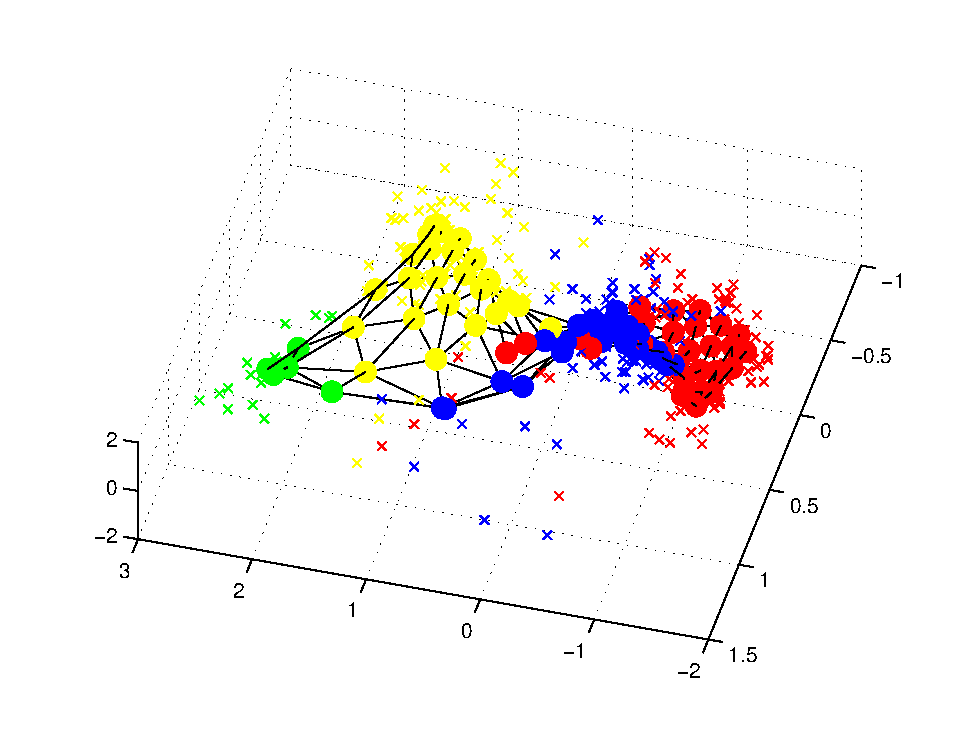
\includegraphics[width=55mm]{som_topol_proj_2}}
  \subfloat[Sammon projection]{\label{fig:som_samon_proj_2}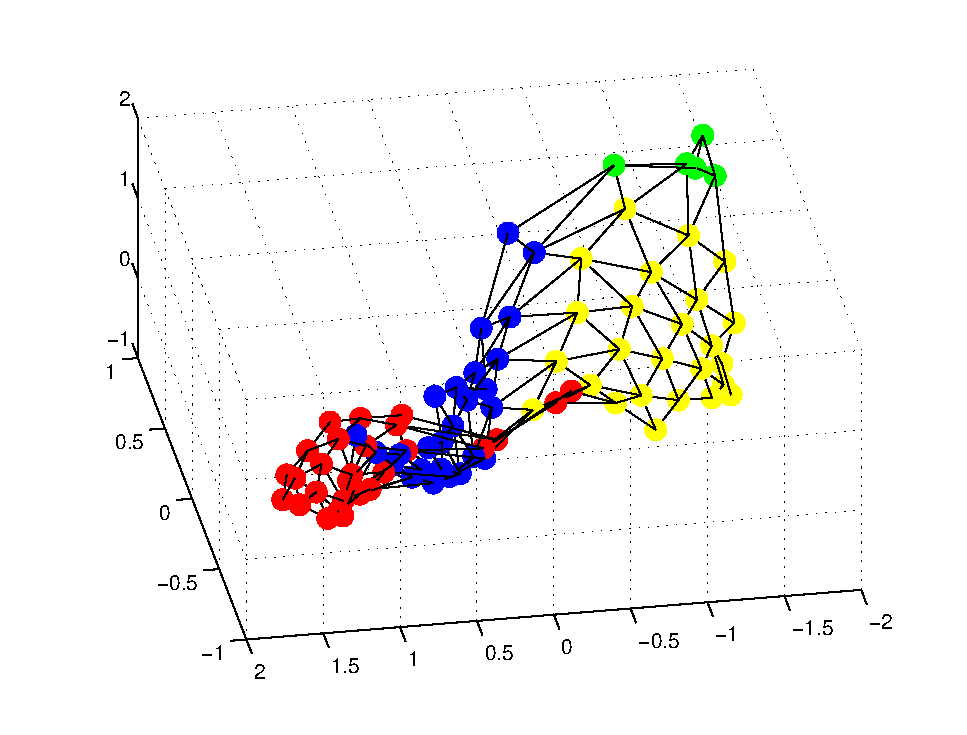
\includegraphics[width=55mm]{som_samon_proj_2}}
  \subfloat[U-matrix and classification]{\label{fig:som_umat_2}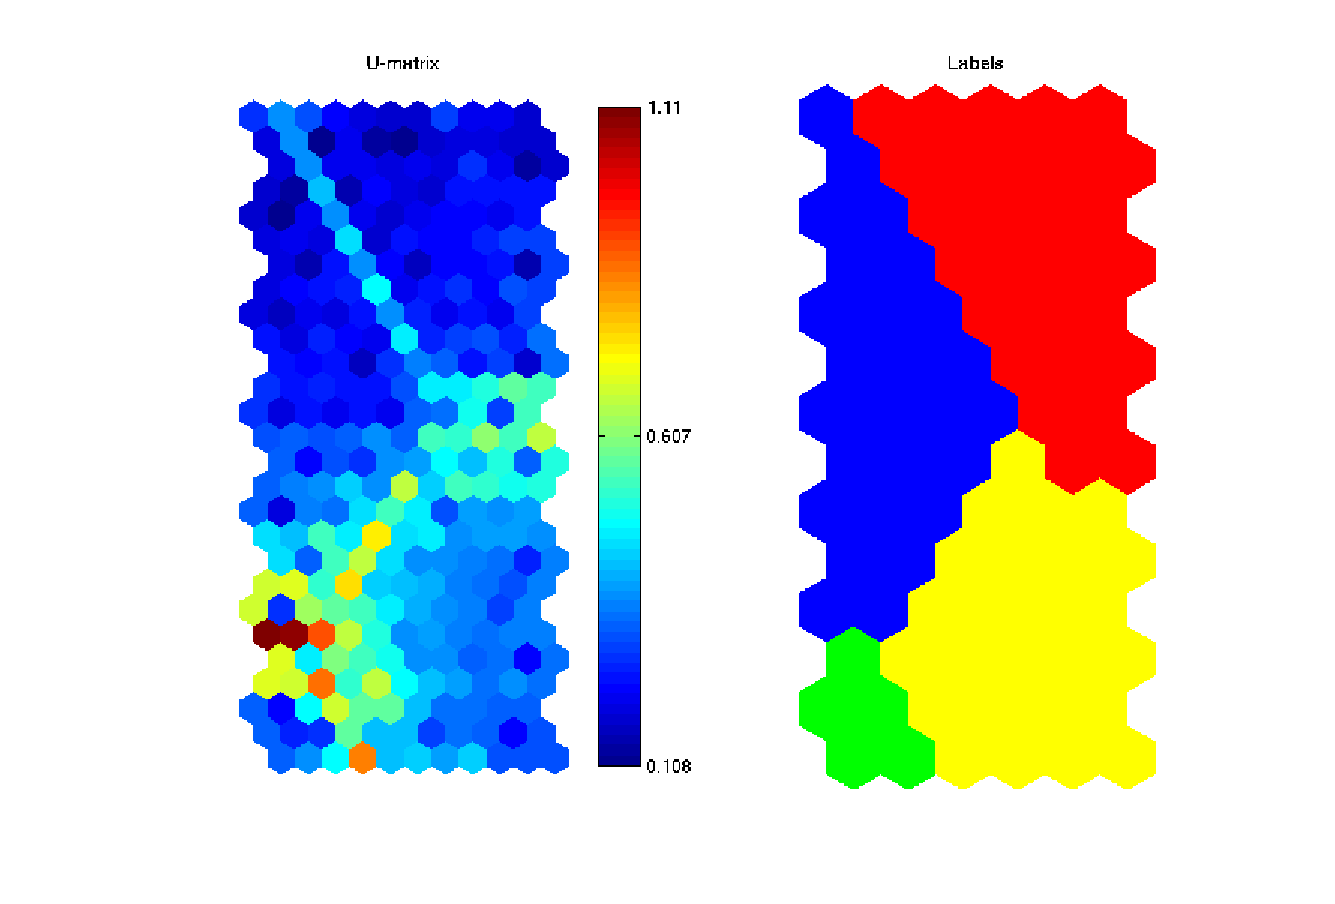
\includegraphics[width=55mm]{som_umat_2}}
  \caption{configuration \#2 (see \textit{tbl. \ref{tbl:somresults}})}
  \label{fig:som_config_2}
\end{figure*}

%\begin{figure*}[!h] %
%  \centering
%  \subfloat[PCA projection]{\label{fig:som_topol_proj_3}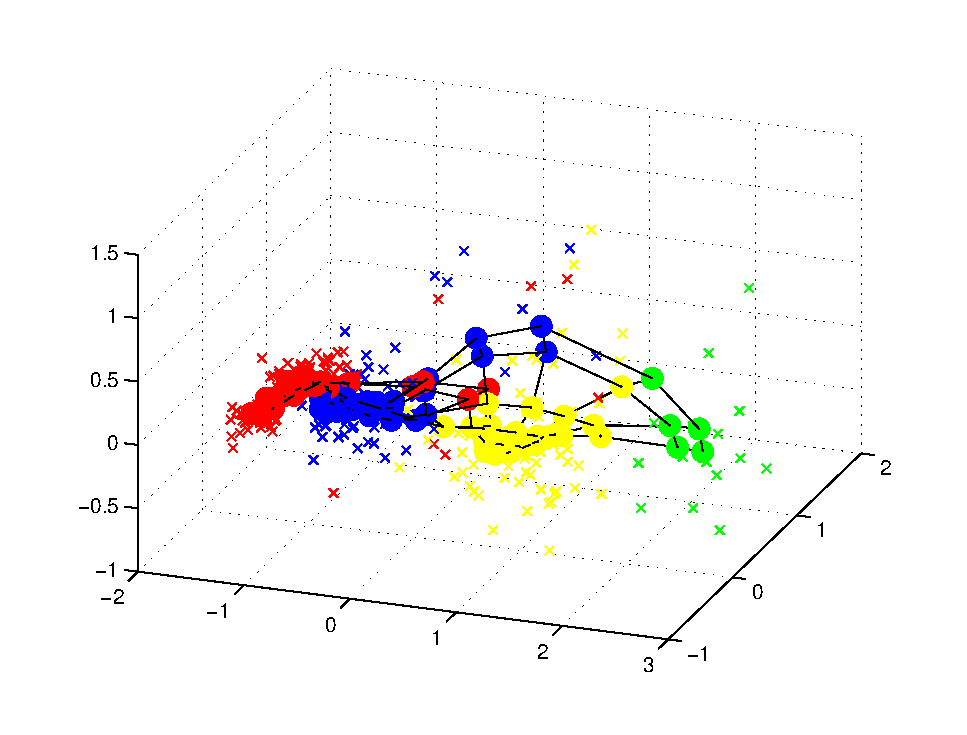
\includegraphics[width=55mm]{som_topol_proj_3}}
%  \subfloat[Sammon projection]{\label{fig:som_samon_proj_3}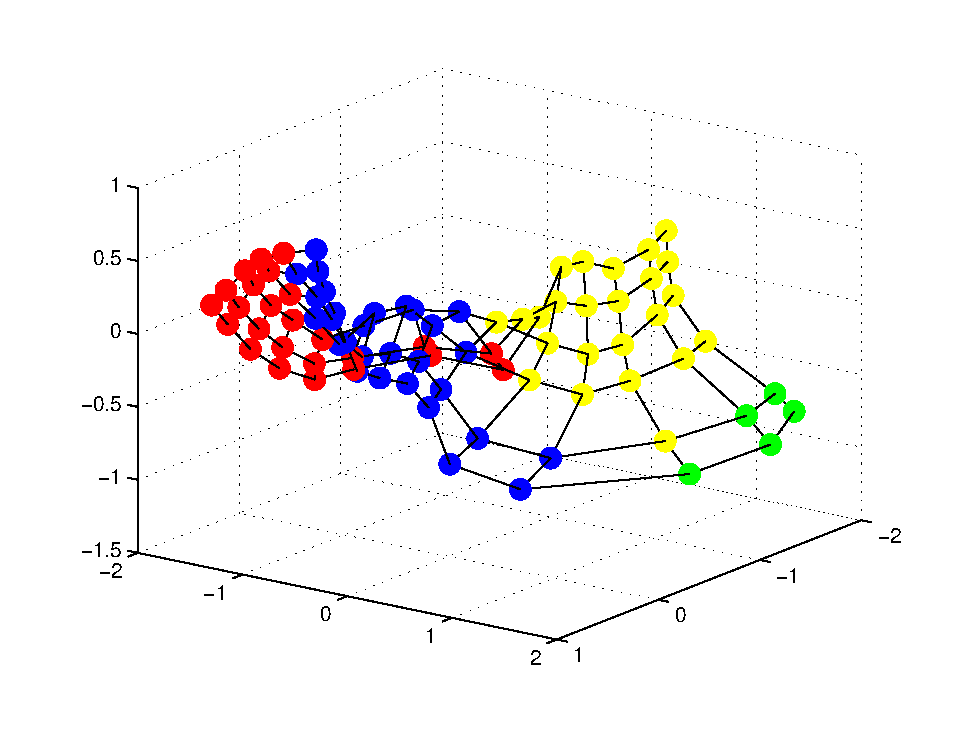
\includegraphics[width=55mm]{som_samon_proj_3}}
%  \subfloat[U-matrix and classification]{\label{fig:som_umat_3}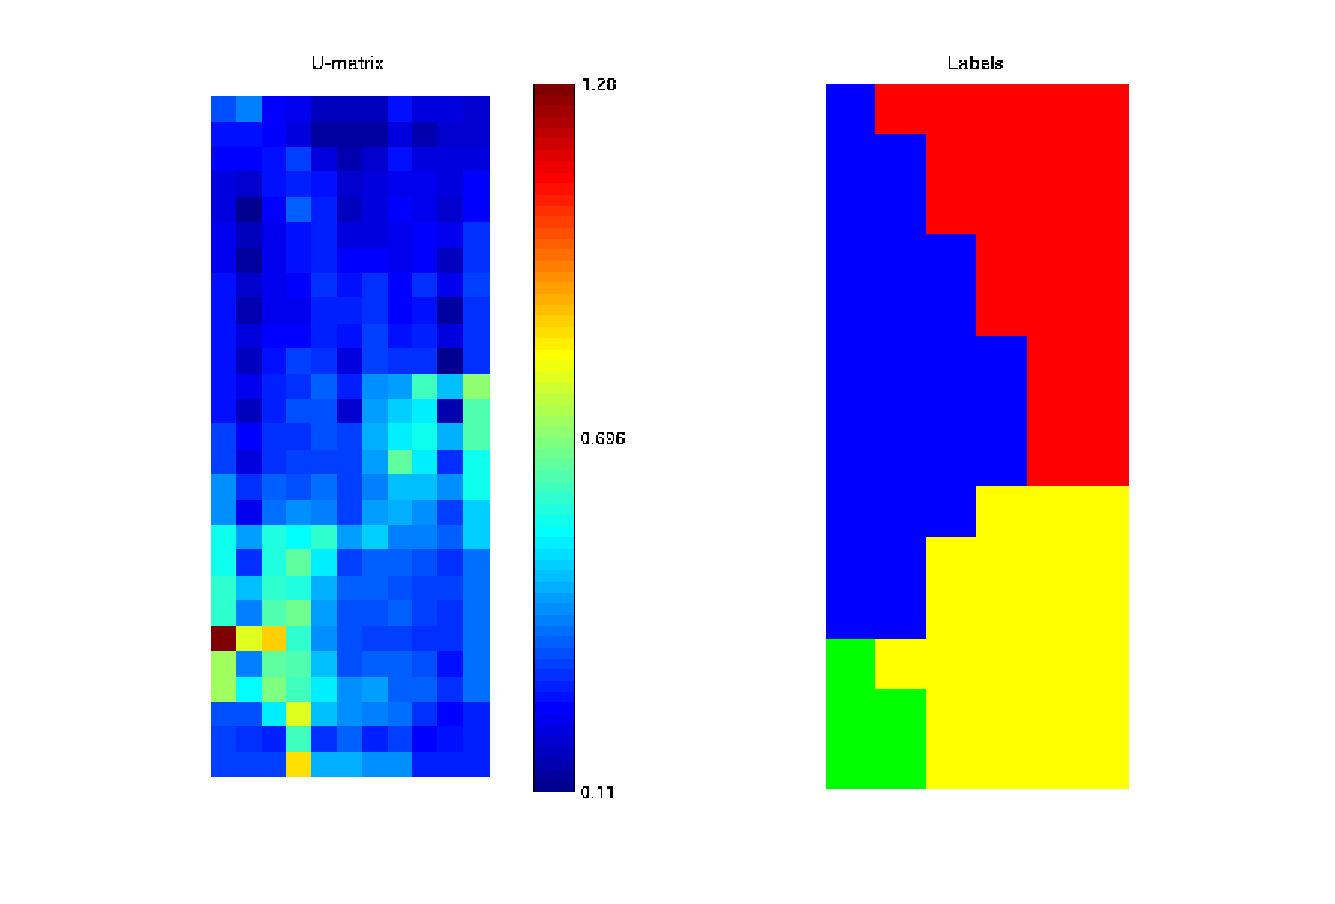
\includegraphics[width=55mm]{som_umat_3}}
%  \caption{configuration \#3 (see \textit{tbl. \ref{tbl:somresults}})}
%  \label{fig:som_config_3}
%\end{figure*}

\begin{figure*}[!h] %
  \centering
  \subfloat[PCA projection]{\label{fig:som_topol_proj_5}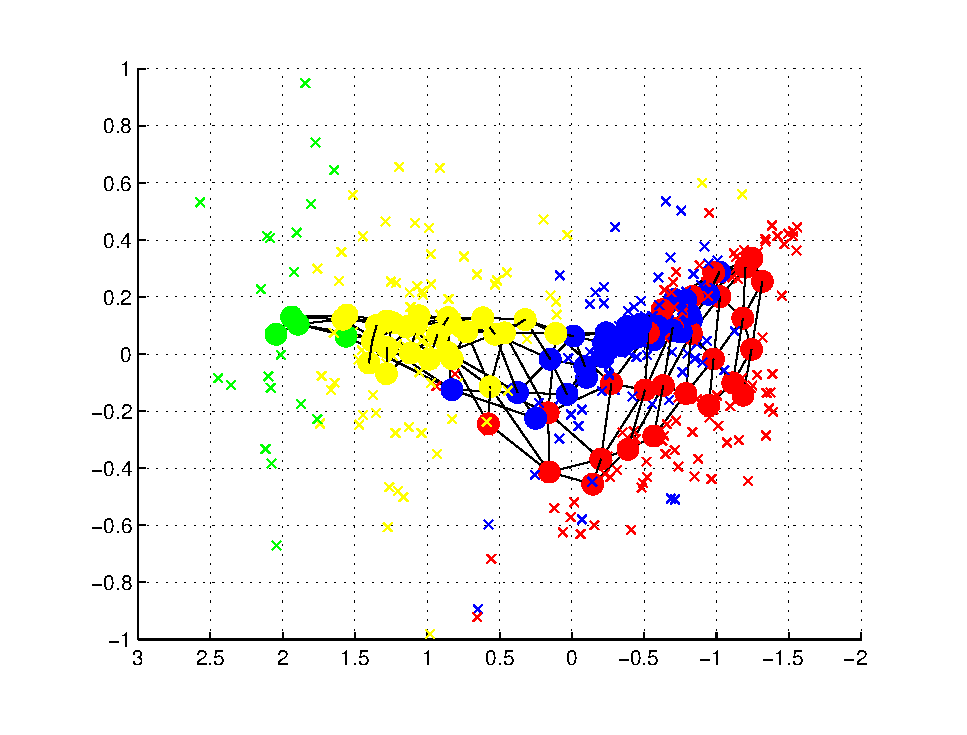
\includegraphics[width=55mm]{som_topol_proj_5}}
  \subfloat[Sammon projection]{\label{fig:som_samon_proj_5}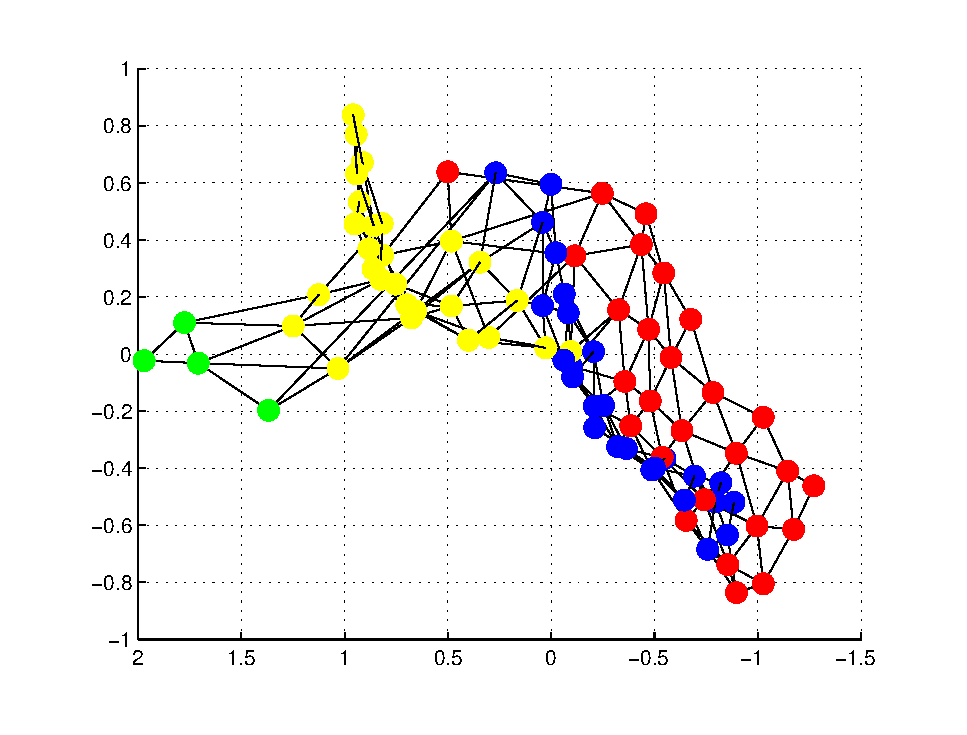
\includegraphics[width=55mm]{som_samon_proj_5}}
  \subfloat[U-matrix and classification]{\label{fig:som_umat_5}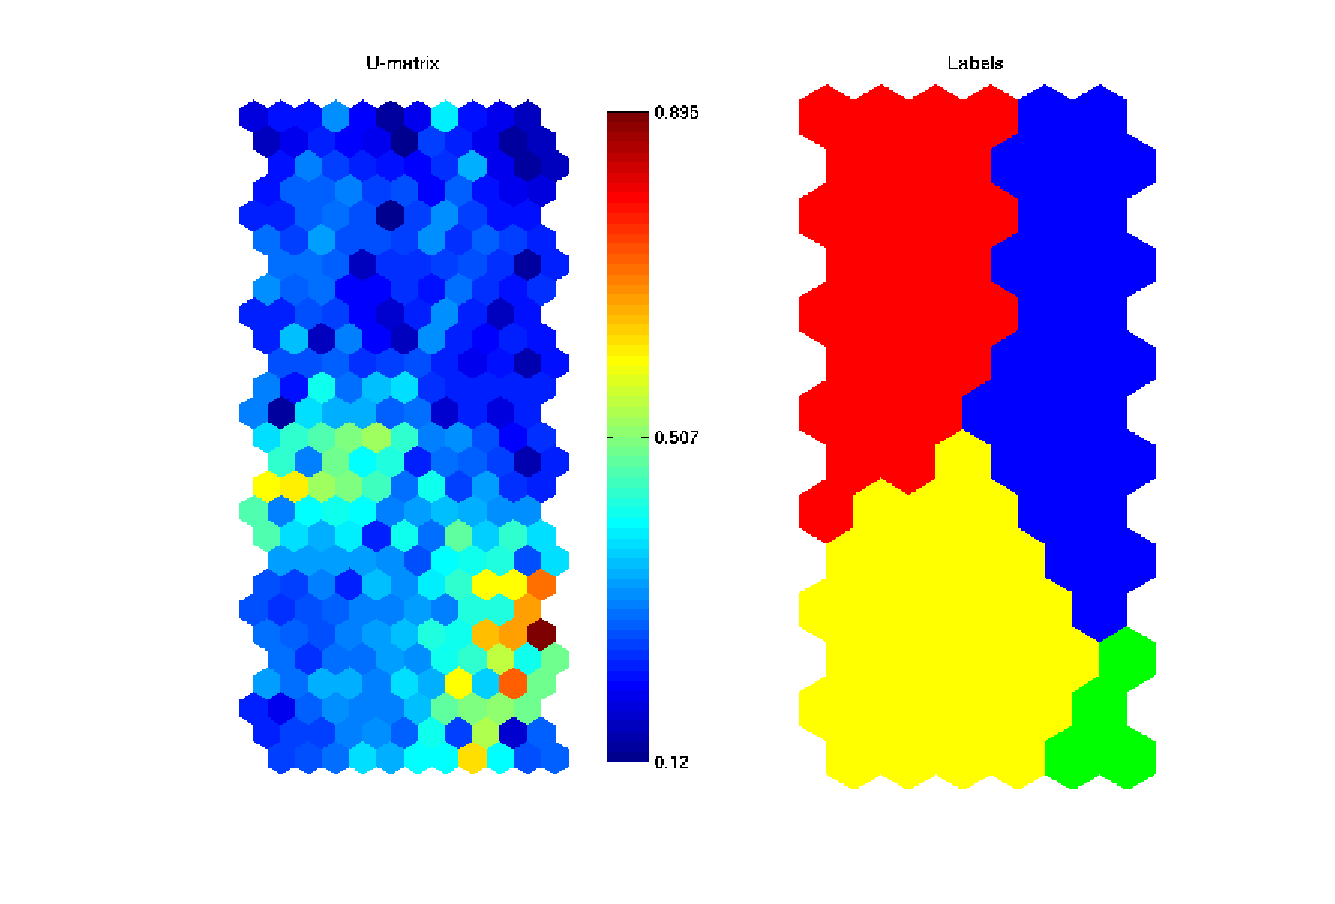
\includegraphics[width=55mm]{som_umat_5}}
  \caption{configuration \#5 (see \textit{tbl. \ref{tbl:somresults}})}
  \label{fig:som_config_5}
\end{figure*}

\begin{figure*}[!h] %
  \centering
  \subfloat[PCA projection]{\label{fig:som_topol_proj_6}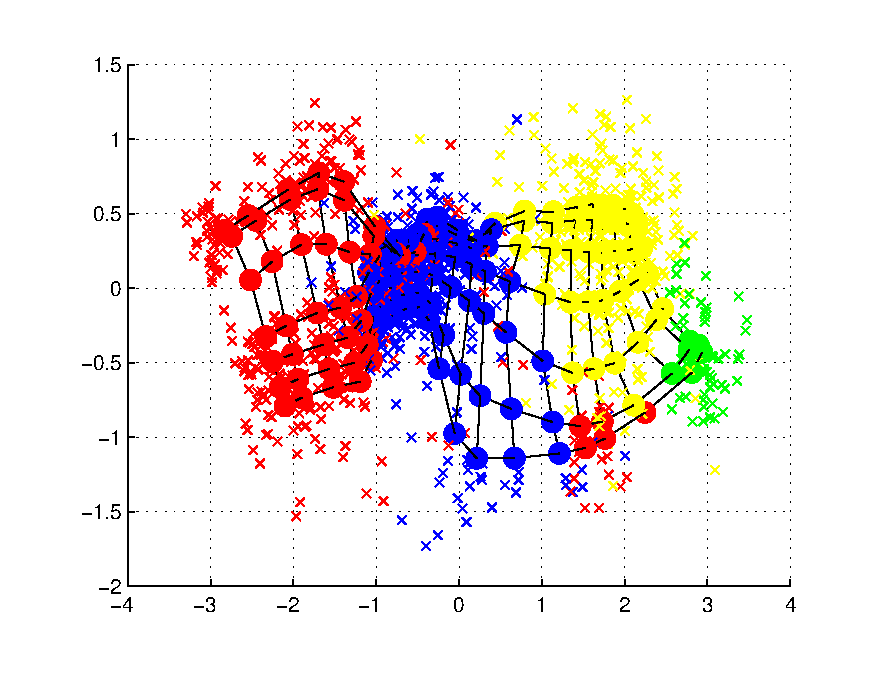
\includegraphics[width=55mm]{som_topol_proj_6}}
  \subfloat[Sammon projection]{\label{fig:som_samon_proj_6}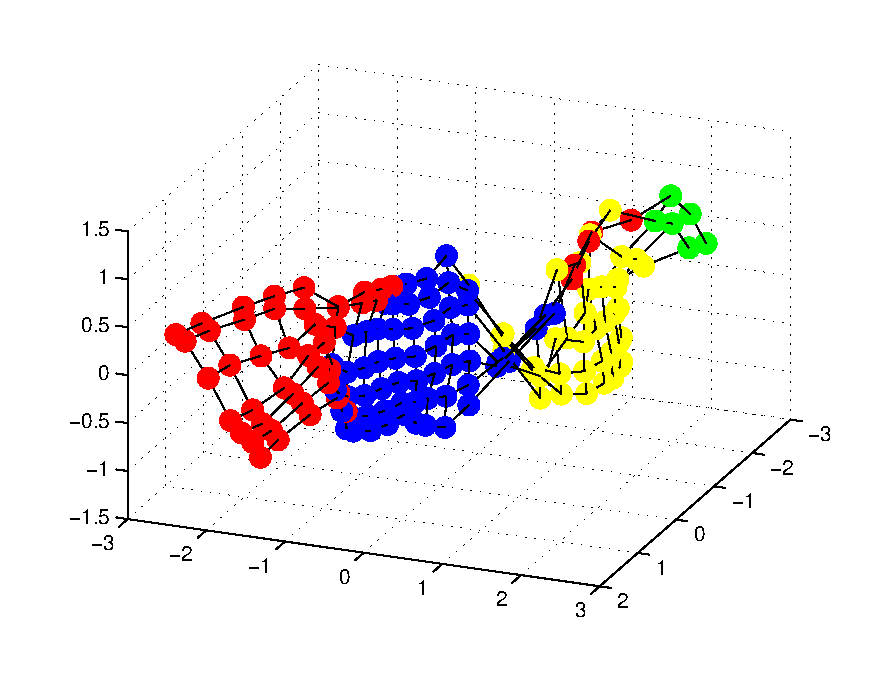
\includegraphics[width=55mm]{som_samon_proj_6}}
  \subfloat[U-matrix and classification]{\label{fig:som_umat_6}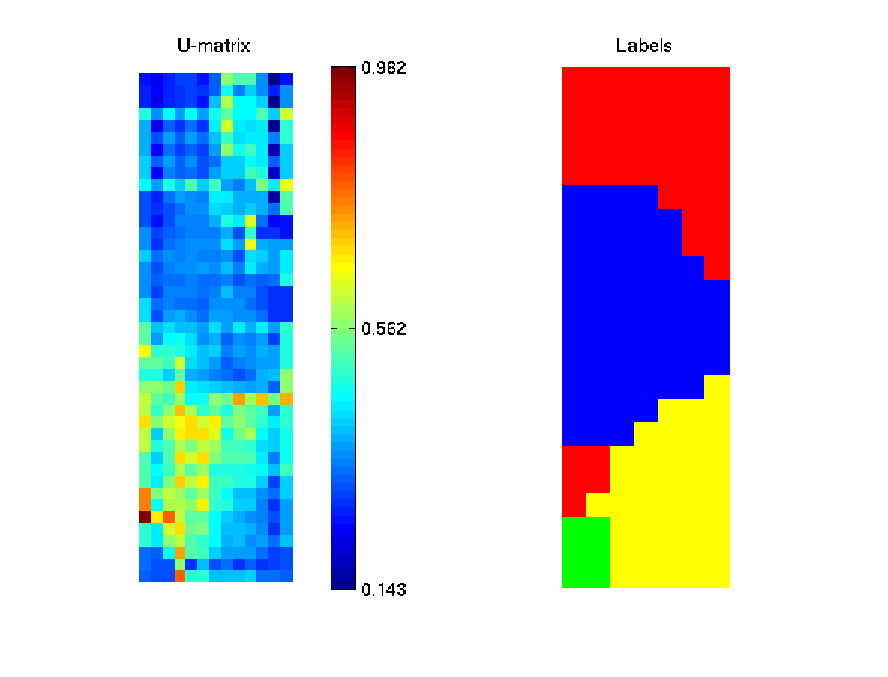
\includegraphics[width=55mm]{som_umat_6}}
  \caption{configuration \#6 (see \textit{tbl. \ref{tbl:somresults}})}
  \label{fig:som_config_6}
\end{figure*}

\begin{figure*}[!h] %
  \centering
  \subfloat[PCA projection]{\label{fig:som_topol_proj_7}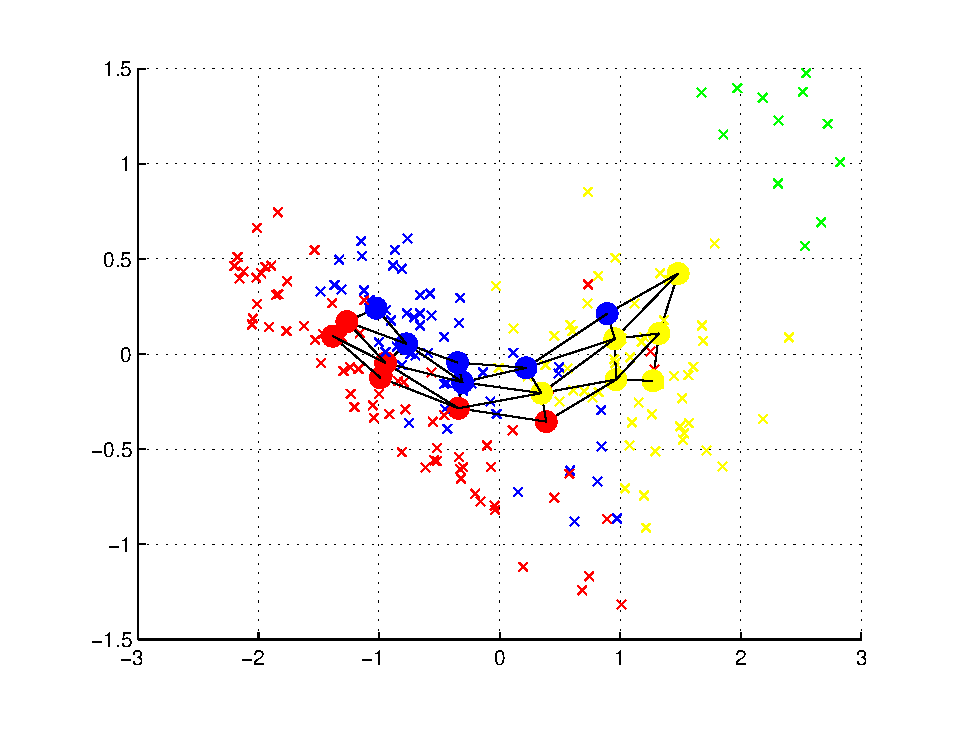
\includegraphics[width=55mm]{som_topol_proj_7}}
  \subfloat[Sammon projection]{\label{fig:som_samon_proj_7}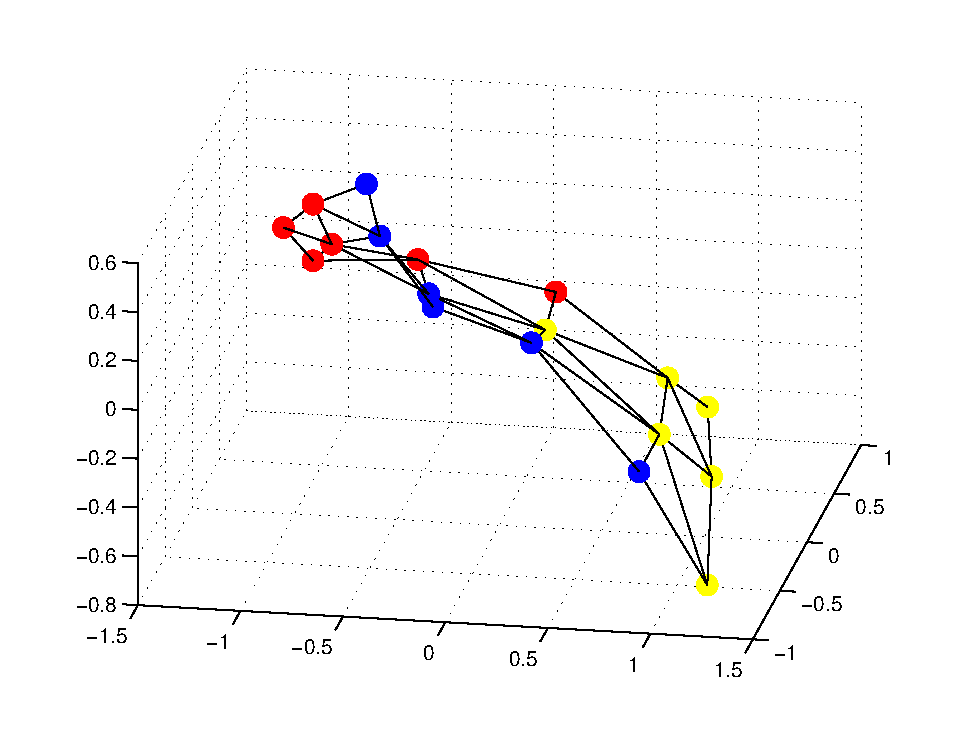
\includegraphics[width=55mm]{som_samon_proj_7}}
  \subfloat[U-matrix and classification]{\label{fig:som_umat_7}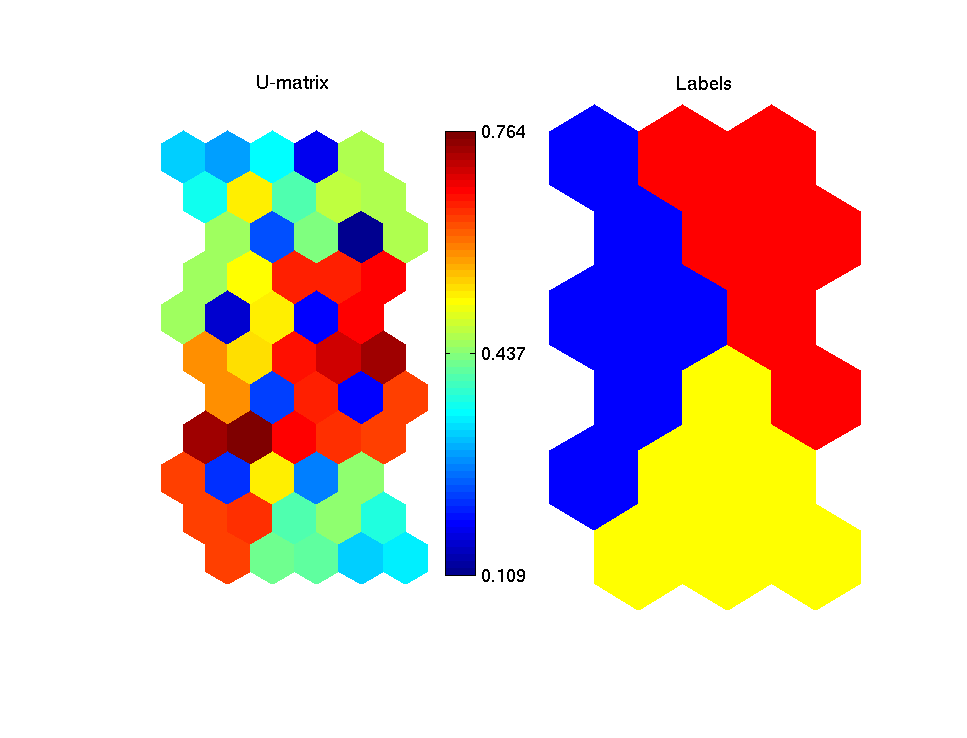
\includegraphics[width=55mm]{som_umat_7}}
  \caption{configuration \#7 (see \textit{tbl. \ref{tbl:somresults}})}
  \label{fig:som_config_7}
\end{figure*}

% that's all folks
\end{document}
